\section{Experimentación}
\subsection{Búsqueda exhaustiva}
Para comenzar la experimentación y tener una idea aproximada sobre los mejores valores de los parámetros del modelo utilizamos la técnica de \textit{grid search} o búsqueda exhaustiva. Siempre corrimos con un \textit{holdout set} de validación del 50\% del dataset completo, para poder simular la performance de nuestra implementación con datos nuevos que no se usaron en el entrenamiento. 

En el ejercicio uno, la búsqueda trata de minimar la suma de errores totales del set de validación, mientras que en el ejercicio dos se hace lo mismo pero al ser un problema de regresión, se define como error cuando el output de la red y el target es mayor a un \textit{epsilon} definido. 

La implementación es bastante simple, lo que hacemos es pasar por parámetro una lista con todos los posibles para parámetros y el algorítmo corre un ciclo, donde en cada ciclo prueba con un parámetro distinto guardandose el mejor modelo para finalmente imprimirlo por la consola. 

Además, se tuvo en cuenta el componente de inicialización aleatorio de la red neuronal. Para esto, decidimos correr 3 veces cada set de parámetros y quedarse con el mejor. 

Los parámetros que variamos fueron los siguientes:
\begin{itemize}
\item \textbf{Learning Rate}
\item \textbf{Momentum}
\item \textbf{Incremental o Batch}
\item \textbf{Configuración/Cantidad de capas y neuronas}
\end{itemize}

Una vez obtenidos los mejores parámetros, continuamos los experimentos variándolos a mano y analizando los resultados. Esto se explicará en la sección siguiente.

El algoritmo es el siguiente:

\begin{lstlisting}[caption=grid\_search]
def grid_search(param_grid):
	grid = ParameterGrid(param_grid)
	best_error = None
	best_params = None
	print "Ejercicio "+str(param_grid["1"])
	print len(grid), "modelos distintos"
	i = 0
	print "i 	error(training, validacion)"
	start = timer()
	for params in grid:
	    e = train(params['1'], params['2'], params['3'],params['4'],params['5'],params['6'],params['7'],
	    	params['8'],params['9'],params['10'],params['11'], True )
	    print i, "	", e
	    i += 1
	    if i%50 == 0:
	    	end = timer()
	    	print int((end-start)/60), " min"
	    if best_error == None or e < best_error:
	    	best_error = e
	    	best_params = [params['1'], params['2'], params['3'],params['4'],params['5'],params['6'],params['7'],params['8'],
	    	params['9'],params['10'],params['11']]
	print "MEJOR ERROR Y MODELO EJERCICIO "+str(param_grid["1"])
	print "training, validacion:", best_error
	print "parametros:", best_params
	end = timer()
	print int((end-start)/60), " min"
\end{lstlisting}

\newpage

Y la forma de instanciarlo es la siguiente:

\begin{lstlisting}[caption=Instanciación]
param_grid = {'1': [1],"2":['./datasets/tp1_ej1_training.csv'],"3": [None], "4":[0.1], "5": [200], 
			"6":[0.001,0.01,0.1,0.5, 0.005, 0.2, 0.3, 0.4], "7":[0.1,0.3,0.5, 0.7, 0.9], "8": [0.70], 
			"9": [0,1], "10":[0], "11":[[5],[10],[15],[20],[25],[15,15],[5,5],[10,10]]}
\end{lstlisting}


\subsection{Ejercicio 1}

Observamos que agregar capas no garantiza la convergencia y, cuando lo hace, provoca que las salidas oscilen abruptamente y tarde más épocas, por lo que optamos por utilizar \textbf{dos capas ocultas} como compromiso entre tiempo y calidad de solución. 

En cuanto al número de unidades por capa, ejecutamos el grid\_search 10 veces y en total encontramos que una buena solución es:

\begin{enumerate}
\item epsilon: 0.1
\item tau: 200
\item etha: 0.01
\item momentum: 0.9
\item holdoutRate: 0.7
\item modo: Incremental
\item unidades por capa: 5 y 5
\end{enumerate}

Y para esta obtuvimos los siguientes graficos.


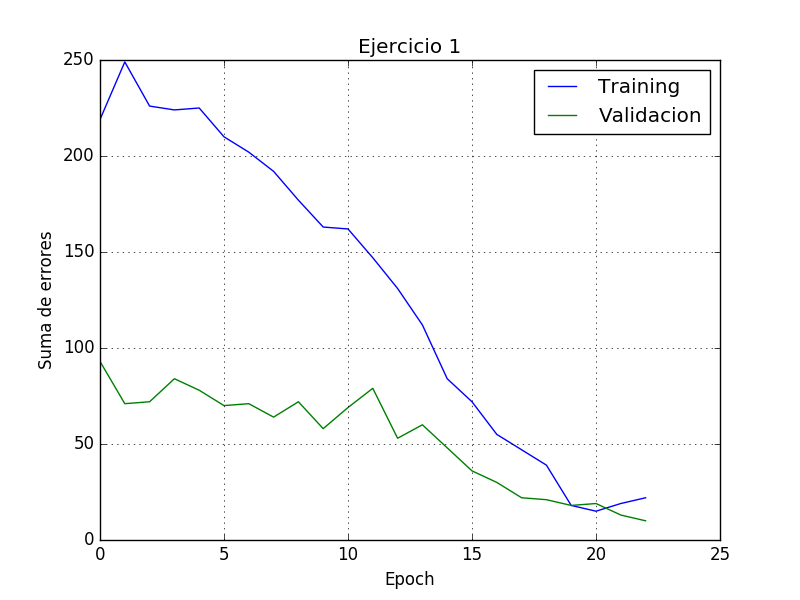
\includegraphics[scale=0.4]{img/ej100109155sum}
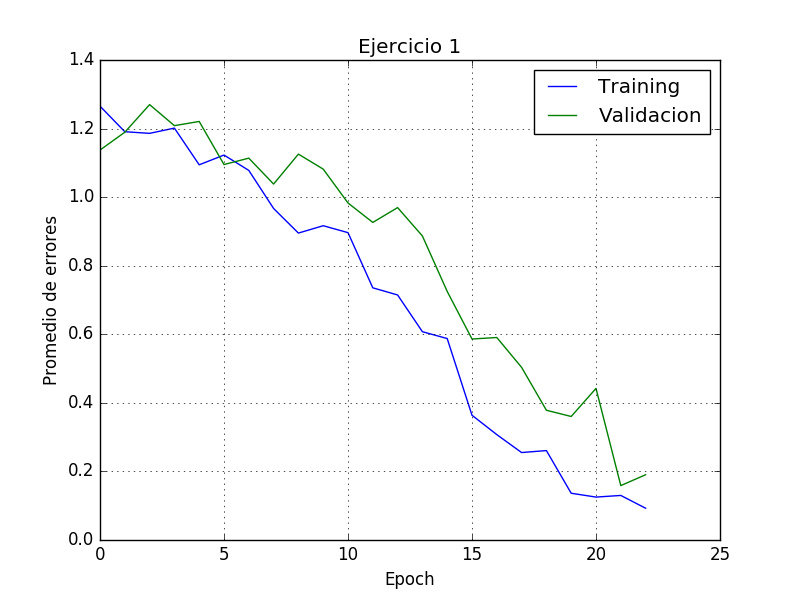
\includegraphics[scale=0.4]{img/ej100109155mean}

En estos gráficos podemos ver que en el promedio, al promediar la cantidad de casos se puede ver que el trainning da mejor que validación. Al mismo tiempo, en la suma de errores la validación da menor porque hay menos casos de entrada. 
Por otro lado, vemos que si mantenemos la cantidad de épocas podemos caer en overfitting porque el error de trainning podría seguir disminuyendo pero el de validación no.

Un detalle importante es que esta arquitectura, cuando convergue, lo hace rápido. Como se pueder ver en este ejemplo de muestra que converge en un poco mas de 20 épocas.

De todas formas, analizando los gráficos tras varias corridas vimos que no siempre converge esta solución.
Como el campo de búsqueda es pequeño, probamos múltiples veces diferentes configuraciones de neuronas con nímeros de 2 a 15 neuronas por capa para tener una evidencia estadística de que sucede al variar este parámetro. Con ello, corroboramos que la solución arrojada por el algoritmo de búsqueda estaba cerca de un resultado optimo al ver las variaciones de diferentes medidas de error. 

Las medidas de error que tomamos fue el número de unidades con error, el error total, el promedio de error, condición de terminación de aprendizaje, es decir, si termino por error menor a epsilon o por límite de épocas. En particular, por la naturaleza del problema, nos interesa ver la Precisión y el Recall, o dicho de otra manera, el índice de falso positivo y falso negativos. 

Como medida utilizaremos la Media armónica donde 

$Media armonica=2*precision*recall/(precision+recall)$

$precision=true positive/(true positive+false positive)$

$recall= true positive/(true positive+false negative)$


Para determinar el valor de la primer capa, elegimos aquellas configuraciones que nunca terminen debido al límite de épocas. Luego, en base a la cantidad de unidades con error y el error total cometido, las clasificamos en este orden. 
En particular, obtuvimos que las configuraciones de [8,7] y [9,5] arrojan buenos resultados (en base a la suma de errores y el promedio).

Podemos ver a continuación algunos gráficos obtenidos variando los parámetros con 8 y 7 capas.

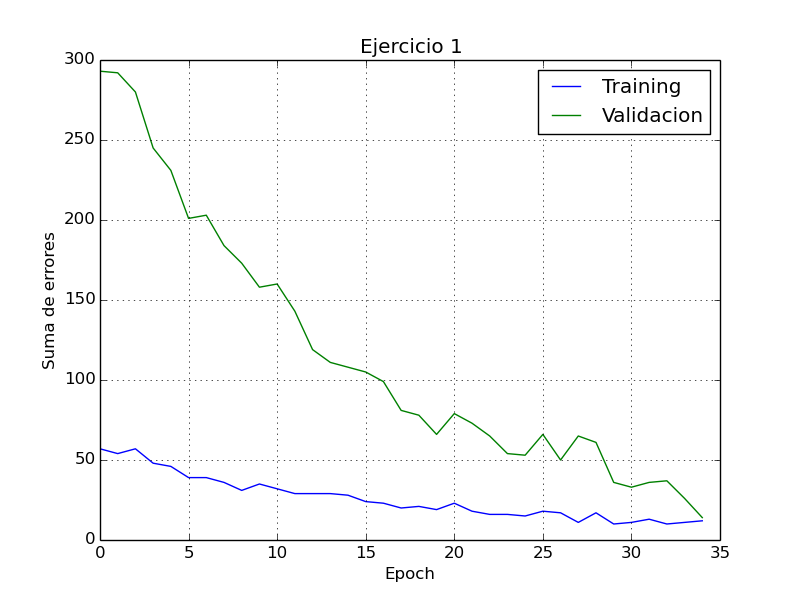
\includegraphics[scale=0.4]{img/ej100207187sum}
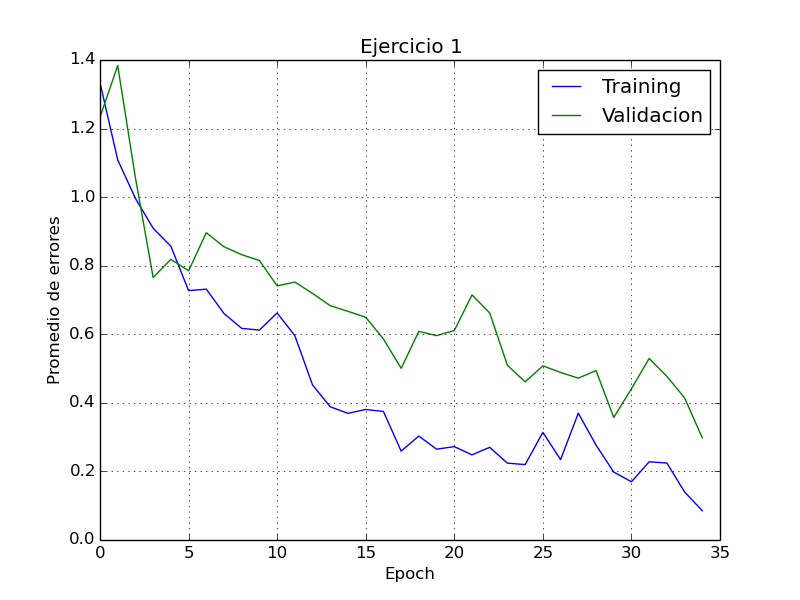
\includegraphics[scale=0.4]{img/ej100207187mean}

En particular este gráfico fue el mejor de los gráficos que obtuvimos variando los parámetros para esta cantidad de capas. Y los parámetros son:
\begin{enumerate}
\item epsilon: 0.1
\item tau: 200
\item etha: 0.02
\item momentum: 0.7
\item holdoutRate: 0.7
\item modo: Incremental
\item unidades por capa: 8 y 7
\end{enumerate}

Se puede ver en estos gráficos que a simple vista, el promedio de errores tiene un mayor número de oscilaciones. También vemos, que comparando a los gráficos del [5,5], este converge en una cantidad de épocas mayor.

\newpage 

Podemos ver a continuación algunos gráficos obtenimos variando los parámetros con 9 y 5 capas.

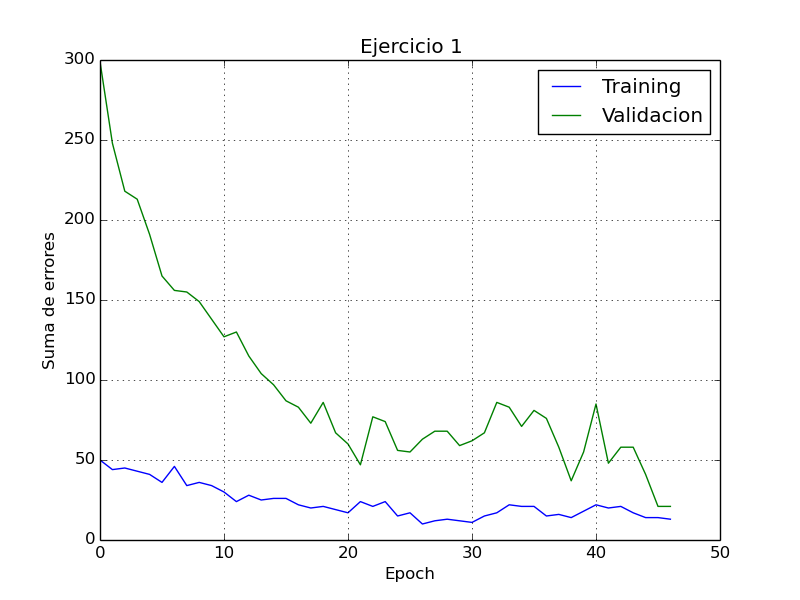
\includegraphics[scale=0.4]{img/ej100505195sum}
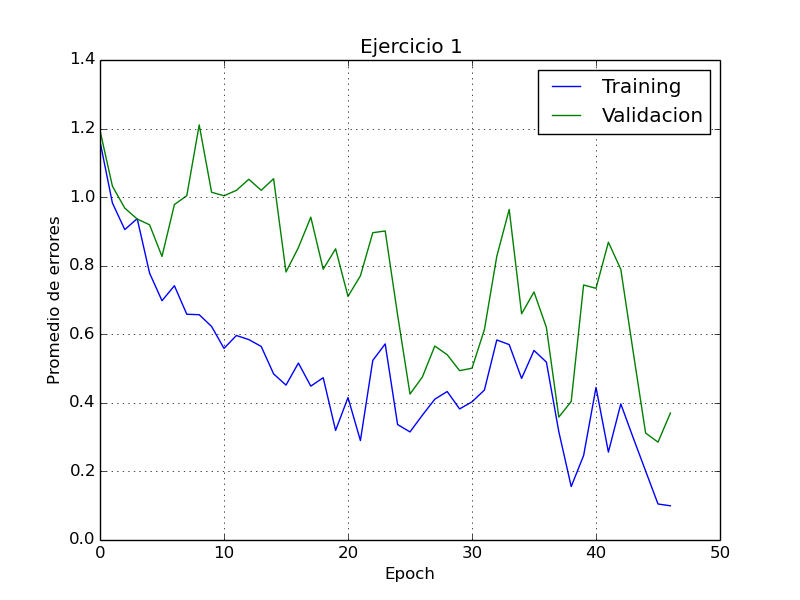
\includegraphics[scale=0.4]{img/ej100505195mean}

En particular, este gráfico fue el mejor de los gráficos que obtuvimos variando los parámetros para esta cantdiad de capas. Y los parámetros son:
\begin{enumerate}
\item epsilon: 0.1
\item tau: 200
\item etha: 0.05
\item momentum: 0.5
\item holdoutRate: 0.7
\item modo: Incremental
\item unidades por capa: 9 y 5
\end{enumerate}

Se puede ver en estos gráficos que el promedio de errores es bastante variado y que al igual que con [8,7] la cantidad de épocas es mayor que [5,5].

Notamos que el número de neuronas en la última capa permite que la salida se ajuste al resultado mientras que la primer capa realiza el grueso del esfuerzo de generalización. Al contrario de lo que esperabamos, incrementar el número de unidades de la última capa no mejora el resultado, si no que lo empeora debido a que le lleva un mayor número de épocas para converger (cuando lo hace). Pocas neuronas en la capa final mostraron experimentalmente que proveen una buena solución.

Por lo mencionado anteriormente, analizamos el valor del Mean Armonic para una muestra que reservamos del dataset original (que no se uso en el entrenamiento) y obtuvimos que el caso de [8,7] capas da un valor del 0.94527, el caso de [9,5] capas da un valor del 0.9508 y el caso de [5,5] capas da un valor de 0.97.

En conclusión, decidimos elegir como modelo el de 5 y 5 capas dado el Mean Armonic da más cercano a 1, es un modelo con pocas capas entonces tiene una velocidad de procesamiento mayor.

\newpage

Además, analizamos los histogramas para ver la cantidad de equivocaciones a la hora de predecir si un cáncer es benigno o maligno obteniendo para el caso de [5,5]:

\begin{center}
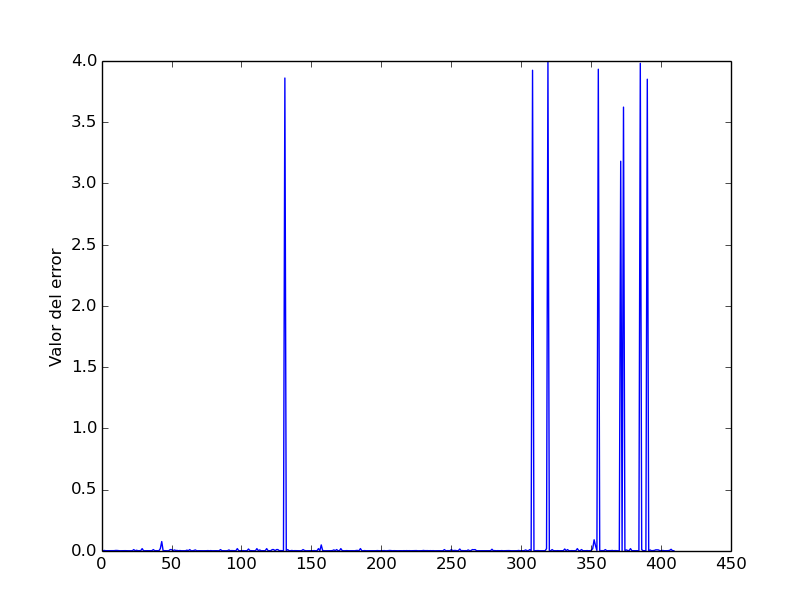
\includegraphics[scale=0.4]{img/histogramaej155}
\end{center}

y para el caso de [9,5] el siguiente gráfico

\begin{center}
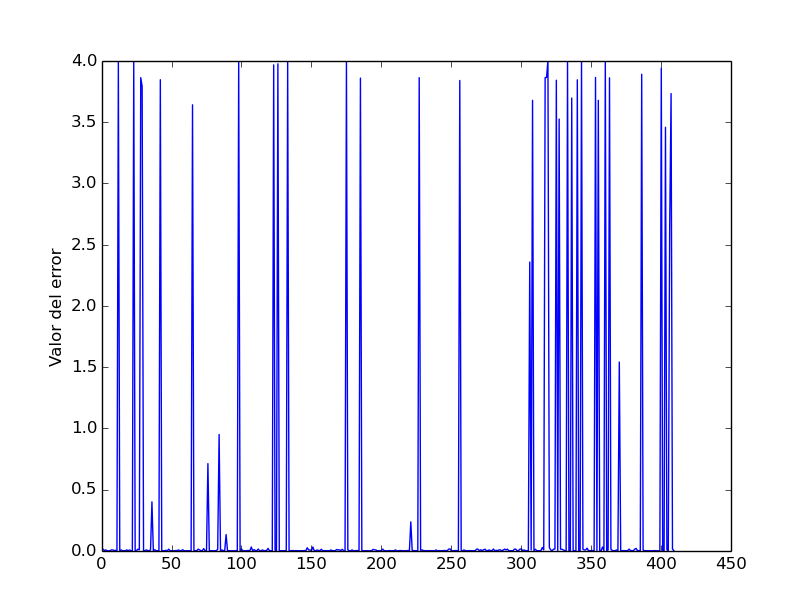
\includegraphics[scale=0.4]{img/ej195_histograma}
\end{center}

Concluyendo, podemos ver que en el gráfico de [5,5] capas la cantidad de equivocaciones es 8, siendo este un número menor que el de [9,5] capas. Tener en cuenta que la cantidad de muestras es de 400.

\newpage

\subsection{Ejercicio 2}

Al igual que en el ejercicio 1, en este ejercicio se corrió el algoritmo de grid\_search 10 veces y en total encontramos dos  soluciones buenas. 

La primera:

\begin{enumerate}
\item epsilon: 0.01
\item tau: 200
\item etha: 0.005
\item momentum: 0.9
\item holdoutRate: 0.7
\item modo: Incremental
\item unidades por capa: 5
\end{enumerate}

Y para esta, obtuvimos los siguientes gráficos.

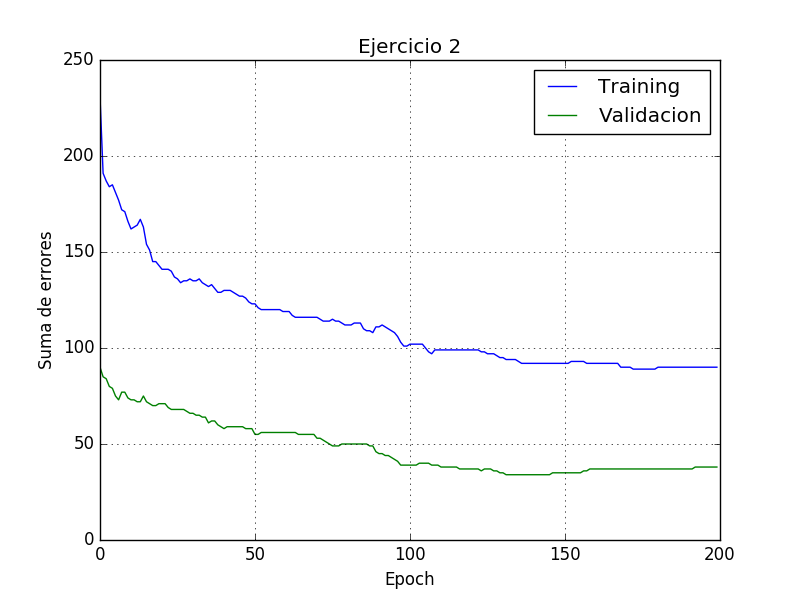
\includegraphics[scale=0.4]{img/ej200050915sum}
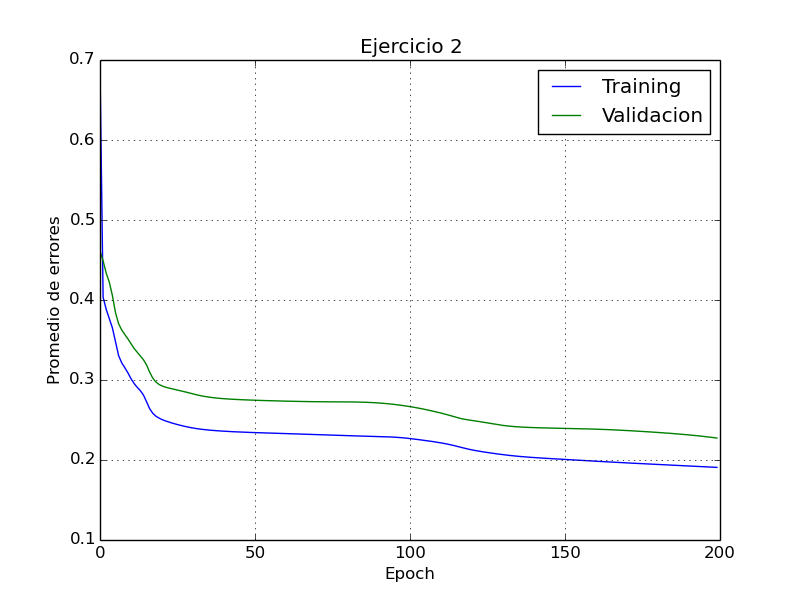
\includegraphics[scale=0.4]{img/ej200050915mean}

Se puede ver en estos gráficos que en el gráfico de suma de errores las dos curvas se comportan igual, esto es porque es un problema de regresión y las funciones utilizadas son linealmente dependiente, es decir, la salida es proporcional a la entrada.

Un detalle importante es que en este gráfico vemos como la curva \textbf{no se plancha}, y este era un problema que teniamos en la mayoria de los casos de 2 capas. 

La otra red que nos arrojo el grid\_search es la siguiente:

\begin{enumerate}
\item epsilon: 0.01
\item tau: 1000
\item etha: 0.01
\item momentum: 0.6
\item holdoutRate: 0.85
\item modo: Incremental
\item unidades por capa: 8 y 5
\end{enumerate}

\newpage

Con esta arquitecutura generamos las siguientes imágenes:

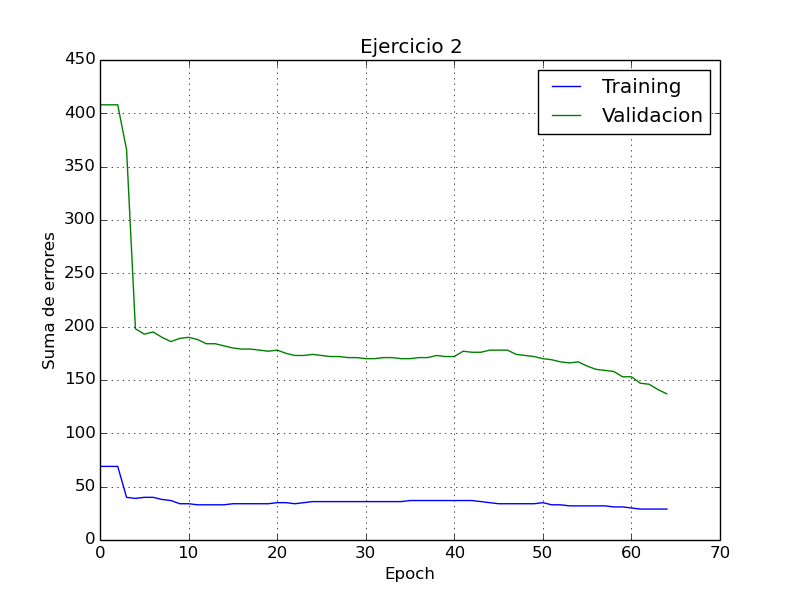
\includegraphics[scale=0.4]{img/asum}
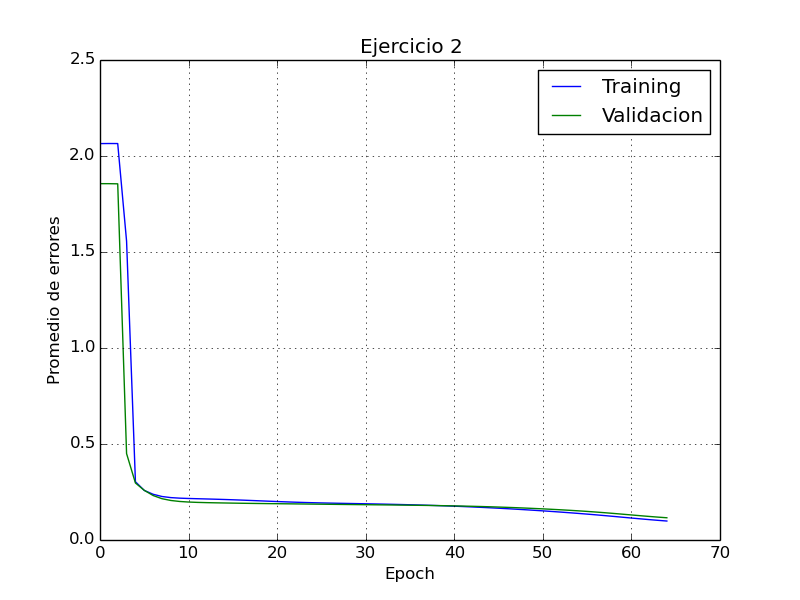
\includegraphics[scale=0.4]{img/bmean}

Se puede ver en estos gráficos que la suma de errores se mantiene constante en un intervalo, es decir, parece que tiene una asintota, en otras palabras, \textbf{se plancha}. Esto es un error típico encontrado en las ejecuciones de 2 capas. Creemos que esto es debido a la función de activación dado que, utilizamos una sidmoide y entonces ésta tiene este comportamiento.

Por otra parte, al igual que en el ejercicio anterior, probamos a mano cambiar los valores de los parámetros pero de todas formas no encontramos nada mejor. En general, todos los resultados que obtuvimos fueron similar a este:

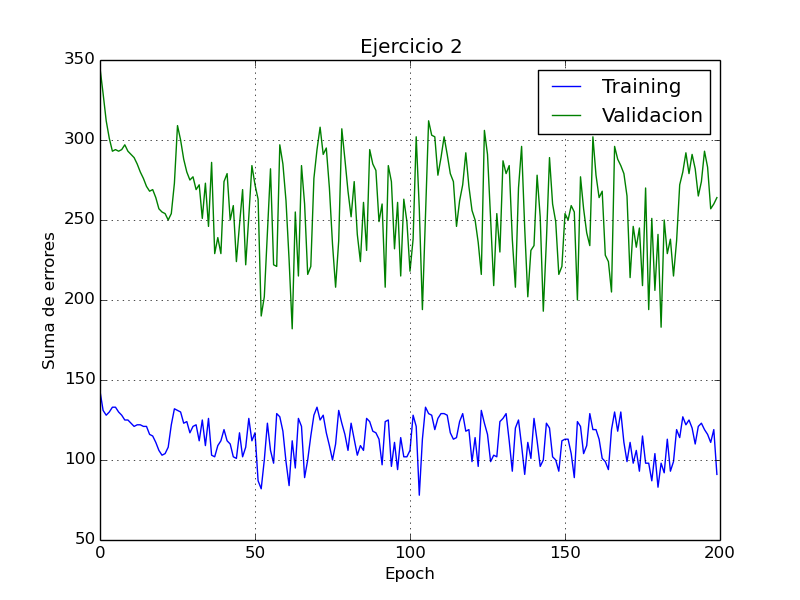
\includegraphics[scale=0.4]{img/ccsum}
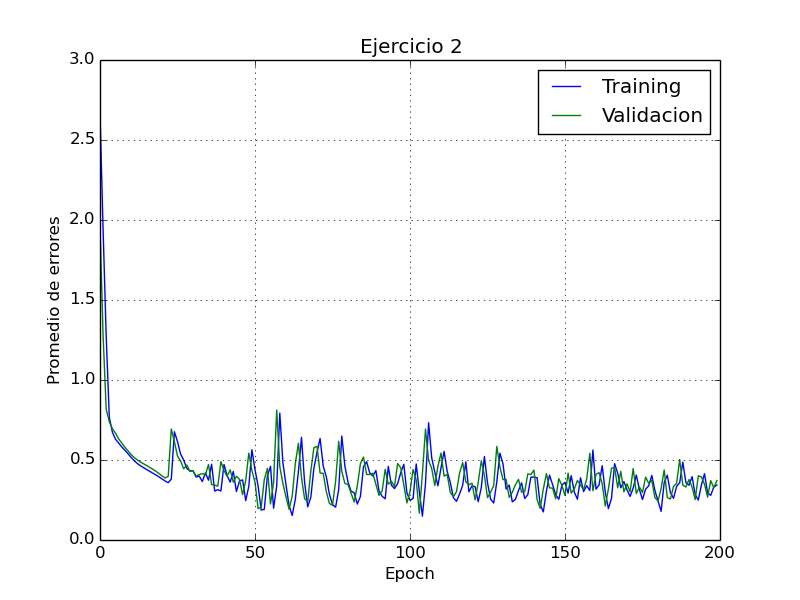
\includegraphics[scale=0.4]{img/bbmean}

estos gráficos corresponden a los siguientes parámetros:

\begin{enumerate}
\item epsilon: 0.01
\item tau: 200
\item etha: 0.1
\item momentum: 0.9
\item holdoutRate: 0.7
\item modo: Batch
\item unidades por capa: 15
\end{enumerate}
En estos gráficos se puede ver una notable inestabilidad por parte de la red (se ve en ambos gráficos). También podemos ver que, la suma de errores se mueve en un intervalo fijo, es decir, no esta descendiendo. 

\newpage

Como se podrá ver en los gráficos elegimos el primer modelo porque es el que mas desciende y también tiene menor cantidad de capas, por lo tanto procesamiento más rapido. También vemos que la derivada de la función de promedio de errores nunca es cero, esto quiere decir que el modelo aprende.

Para este modelo elegido, hicimos unos gráficos de disperción. 

En este gráfico se puede ver en el eje \textbf{y} el valor predicho y en el eje \textbf{x} el valor objetivo. En general lo ideal es concluir en un grafico como el siguiente:

\begin{center}
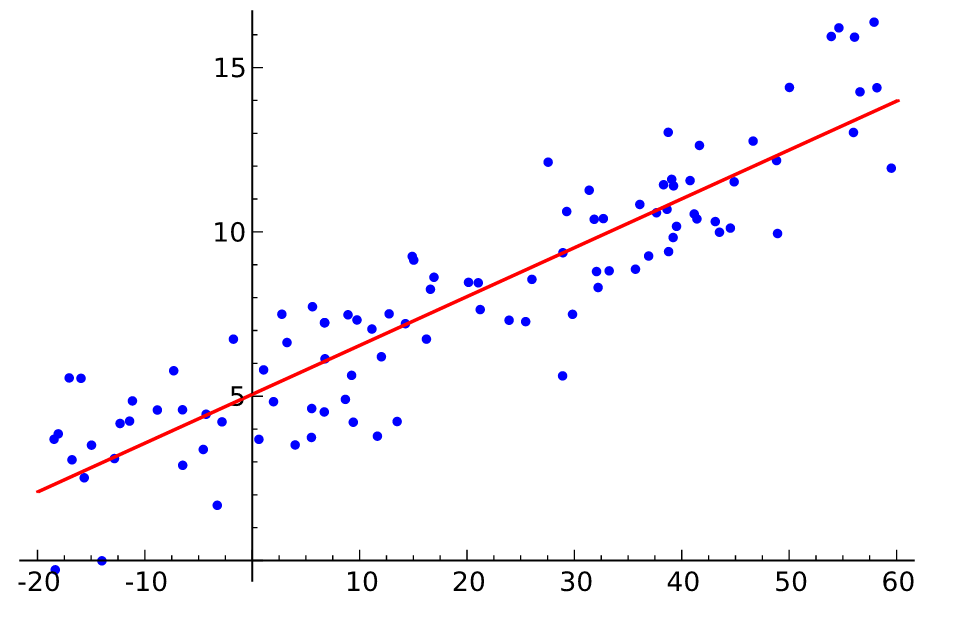
\includegraphics[scale=0.4]{img/regresionperfecta}
\end{center}

Con nuestra arquitectura obtuvimos los siguientes gráficos:

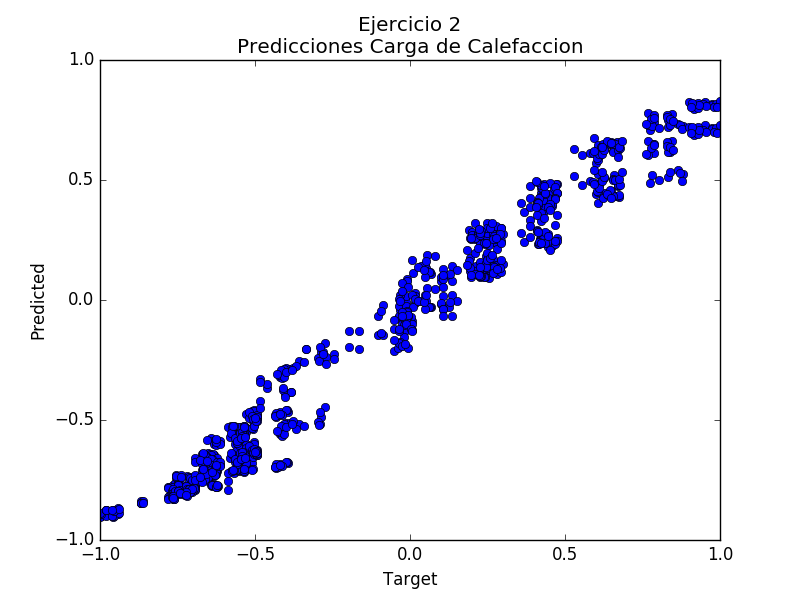
\includegraphics[scale=0.4]{img/ej2-calef}
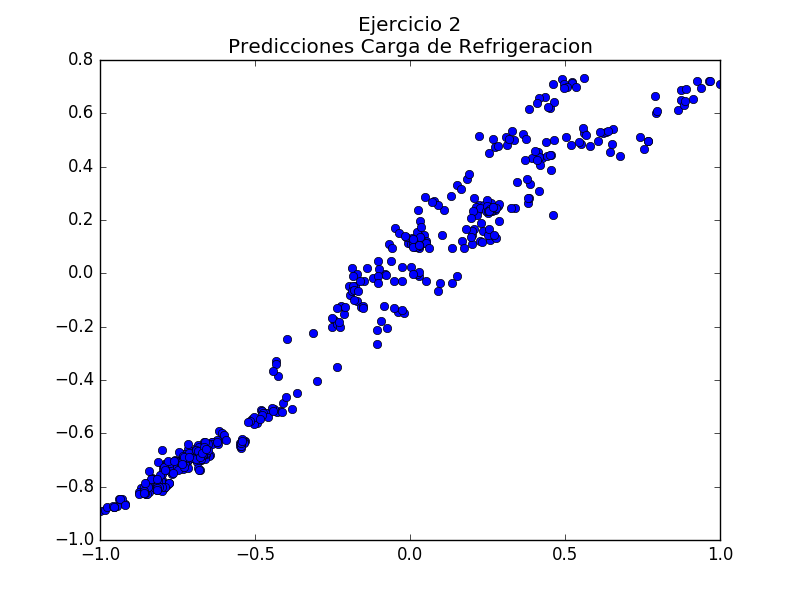
\includegraphics[scale=0.4]{img/ej2-refrig}


En estos gráficos notamos que son similares a lo ideal, sin caer en un overfitting, los puntos obtenidos se acercan a la recta Y=X, lo que quiere decir que los valores aprendidos se acercan mucho al objetivo.

Como se explicó en las secciones anteriores el output fue normalizado, por esto la escala del gráfico va desde -1 a 1 que es el rango de la función sigmoide bipolar.
